\documentclass[hyperref, a4paper]{article}

\usepackage{geometry}
\usepackage{titling}
\usepackage{titlesec}
% No longer needed, since we will use enumitem package
% \usepackage{paralist}
\usepackage{enumitem}
\usepackage{footnote}
\usepackage{amsmath, amssymb, amsthm}
\usepackage{mathtools}
\usepackage{bbm}
\usepackage{graphicx}
\usepackage{subcaption}
\usepackage{physics}
\usepackage{tensor}
\usepackage{siunitx}
\usepackage[version=4]{mhchem}
\usepackage{tikz}
\usepackage{xcolor}
\usepackage{listings}
\usepackage{autobreak}
\usepackage[ruled, vlined, linesnumbered]{algorithm2e}
\usepackage[backend=bibtex]{biblatex}
\addbibresource{data.bib}
\addbibresource{experiments.bib}
\addbibresource{theory.bib}
\usepackage[colorlinks,unicode]{hyperref} % , linkcolor=black, anchorcolor=black, citecolor=black, urlcolor=black, filecolor=black
\usepackage[most]{tcolorbox}
\usepackage{prettyref}

% Page style
\geometry{left=3.18cm,right=3.18cm,top=2.54cm,bottom=2.54cm}
\titlespacing{\paragraph}{0pt}{1pt}{10pt}[20pt]
\setlength{\droptitle}{-5em}

% More compact lists 
\setlist[itemize]{
    itemindent=17pt, 
    leftmargin=1pt,
    listparindent=\parindent,
    parsep=0pt,
}

% Math operators
\DeclareMathOperator{\timeorder}{\mathcal{T}}
\DeclareMathOperator{\diag}{diag}
\DeclareMathOperator{\legpoly}{P}
\DeclareMathOperator{\primevalue}{P}
\DeclareMathOperator{\sgn}{sgn}
\DeclareMathOperator{\res}{Res}
\newcommand*{\ii}{\mathrm{i}}
\newcommand*{\ee}{\mathrm{e}}
\newcommand*{\const}{\mathrm{const}}
\newcommand*{\suchthat}{\quad \text{s.t.} \quad}
\newcommand*{\argmin}{\arg\min}
\newcommand*{\argmax}{\arg\max}
\newcommand*{\normalorder}[1]{: #1 :}
\newcommand*{\pair}[1]{\langle #1 \rangle}
\newcommand*{\fd}[1]{\mathcal{D} #1}
\DeclareMathOperator{\bigO}{\mathcal{O}}

% TikZ setting
\usetikzlibrary{calc}
\usetikzlibrary{arrows,shapes,positioning}
\usetikzlibrary{arrows.meta}
\usetikzlibrary{decorations.markings}
\tikzstyle arrowstyle=[scale=1]
\tikzstyle directed=[postaction={decorate,decoration={markings,
    mark=at position .5 with {\arrow[arrowstyle]{stealth}}}}]
\tikzstyle ray=[directed, thick]
\tikzstyle dot=[anchor=base,fill,circle,inner sep=1pt]

% Algorithm setting
% Julia-style code
\SetKwIF{If}{ElseIf}{Else}{if}{}{elseif}{else}{end}
\SetKwFor{For}{for}{}{end}
\SetKwFor{While}{while}{}{end}
\SetKwProg{Function}{function}{}{end}
\SetArgSty{textnormal}

\newcommand*{\concept}[1]{{\textbf{#1}}}

% Embedded codes
\lstset{basicstyle=\ttfamily,
  showstringspaces=false,
  commentstyle=\color{gray},
  keywordstyle=\color{blue}
}

% Reference formatting
\newrefformat{fig}{Fig.~\ref{#1}}
\newcommand*{\term}[1]{\textit{#1}}

% Color boxes
\tcbuselibrary{skins, breakable, theorems}

\newtcbtheorem[number within=section]{infobox}{Box}{
    enhanced,
    boxrule=0pt,
    colback=blue!5,
    colframe=blue!5,
    coltitle=blue!50,
    borderline west={4pt}{0pt}{blue!65},
    sharp corners,
    fonttitle=\bfseries, 
    breakable,
    before upper={\parindent15pt\noindent}}{box}
\newtcbtheorem[number within=section, use counter from=infobox]{theorybox}{Box}{
    enhanced,
    boxrule=0pt,
    colback=orange!5, 
    colframe=orange!5, 
    coltitle=orange!50,
    borderline west={4pt}{0pt}{orange!65},
    sharp corners,
    fonttitle=\bfseries, 
    breakable,
    before upper={\parindent15pt\noindent}}{box}
\newtcbtheorem[number within=section, use counter from=infobox]{learnbox}{Box}{
    enhanced,
    boxrule=0pt,
    colback=green!5,
    colframe=green!5,
    coltitle=green!50,
    borderline west={4pt}{0pt}{green!65},
    sharp corners,
    fonttitle=\bfseries, 
    breakable,
    before upper={\parindent15pt\noindent}}{box}

% Displaying texts in bookmarkers

\pdfstringdefDisableCommands{%
  \def\\{}%
  \def\ce#1{<#1>}%
}

\pdfstringdefDisableCommands{%
  \def\texttt#1{<#1>}%
  \def\mathbb#1{#1}%
}
\pdfstringdefDisableCommands{\def\eqref#1{(\ref{#1})}}

\makeatletter
\pdfstringdefDisableCommands{\let\HyPsd@CatcodeWarning\@gobble}
\makeatother

\newenvironment{shelldisplay}{\begin{lstlisting}}{\end{lstlisting}}

\newcommand*{\efermi}{E_{\text{F}}}
\newcommand*{\sA}{\text{A}}
\newcommand*{\sB}{\text{B}}
\newcommand*{\Tc}{T_{\text{c}}}
\newcommand*{\muB}{\mu_{\text{B}}}
\newcommand*{\kB}{k_{\text{B}}}

\setlength{\fboxrule}{0.1pt}
\newcommand*\up{\fbox{$\mathord\upharpoonleft\phantom{\downharpoonright}$}}%
\newcommand*\dn{\fbox{$\mathord\downharpoonleft\phantom{\upharpoonright}$}}%
\newcommand*\updn{\fbox{$\upharpoonleft\downharpoonright$}}%
\newcommand*\emp{\fbox{$\phantom{\downharpoonright}\phantom{\downharpoonright}$}}%
\newcommand{\electron}[2]{{%
        \setlength\tabcolsep{0pt}% remove extra horizontal space from tabular
%       \setlength\fboxrule{0.2pt}% uncomment for original line width
        \begin{tabular}{c}
            \fboxsep=0pt\fbox{\fboxsep=3pt#2}\\[2pt]
            #1
        \end{tabular}%
}}

\title{Midterm}
\author{Jinyuan Wu}

\begin{document}

\maketitle

\section{Problem 1}

\subsection{}

The electron configuration of \ce{Fe} is [Ar]3d$^6$4s$^2$,
and according to Hund's rule, 
the spins are 
\begin{center}
    \electron{3d}{\updn \up \up \up \up} \electron{4s}{\updn}
\end{center}
The electron configuration of \ce{Fe^{2+}} is [Ar]3d$^6$,
and according to Hund's rule, 
the spins are 
\begin{center}  
    \electron{3d}{\updn \up \up \up \up}
\end{center}
\ce{Fe^{3+}} is obtained by reducing one electron and the spins are 
\begin{center}
    \electron{3d}{\up \up \up \up \up}
\end{center}

For an iron atom,
we only need to work on the 3d orbital 
because the 4s orbital is full.
the total spin quantum number is $S = 2$,
and the total orbital angular momentum quantum number is $L = 2$.
Therefore 
\begin{equation}
    g_J = \frac{3}{2} + \frac{S(S+1) - L(L+1)}{2J(J+1)} = \frac{3}{2}.
\end{equation}
Since the 3d shell is more than half filled, 
we have $J = L + S = 4$,
and the total magnetic moment should be 
\begin{equation}
    \mu = \muB g_J J = 6 \muB.
\end{equation}

\subsection{}

The experimentally observed atomic magnetic moment is $2.22\muB$,
which doesn't agree with the aforementioned prediction.
If somehow the orbital angular momentum is quenched, 
then $S = J = 2$,
and $g_J = 2$.
So the total angular momentum is $2$, which is close to $2.22$,
but $g_J$ should be multiplied to the former
and the result $4 \muB$ is no longer close to $2.22 \muB$.
The predicted $4 \muB$ magnetic moment however 
agrees well with the $4.4 \muB$ magnetic moment 
of \ce{Fe^{2+}} \cite{PhysRevB.63.172404},
which should have the same magnetic moment with Fe atom
because in both of them, only the 3d orbital is open.

\subsection{}

$\alpha$-\ce{Fe} has a bcc structure;
and the lattice constant is \SI{2.86}{\angstrom}
(this can be found with MaterialProject).
So there are 8 nearest atoms for each iron atom.
The distance between two nearest neighbor iron atoms is 
\[
    \SI{2.86}{\angstrom} \cdot \frac{\sqrt{3}}{2} = \SI{2.48}{\angstrom}.
\]

\subsection{}

We work in Hartree atomic units.
Since the exact many-body wave function of a iron atom is hard to obtain,
as an estimation of magnitude, 
we place only one electron on each iron atom,
the wave function of which is 
\begin{equation}
    \varphi(\vb*{r}) = A r^2 \ee^{-r/2}.
\end{equation}
The wave function is normalized as 
\begin{equation}
    A^2 \cdot 4 \pi \cdot \int_{0}^{\infty} r^2 \dd{r} r^4 \ee^{-r} = 1 \Rightarrow
    A = \frac{1}{24 \sqrt{5\pi}}.
\end{equation}
Suppose $a$ is the distance between two iron atoms.
We have 
\begin{equation}
    \begin{aligned}
        J &= \int \dd[3]{\vb*{r}_1} \int \dd[3]{\vb*{r}_2} 
        \varphi^*_2(\vb*{r}_1) \varphi_1(\vb*{r}_1) 
        \frac{1}{\abs*{\vb*{r}_1 - \vb*{r}_2}} 
        \varphi_1^*(\vb*{r}_2) \varphi_2(\vb*{r}_2) \\
        &= \int \dd[3]{\vb*{r}_1} \int \dd[3]{\vb*{r}_2} 
        \varphi(\vb*{r}_1 - a \vu*{x} / 2) \varphi(\vb*{r}_1 + a \vu*{x} / 2) 
        \frac{1}{\abs*{\vb*{r}_1 - \vb*{r}_2}} 
        \varphi(\vb*{r}_2 + a \vu*{x} / 2) \varphi(\vb*{r}_2 - a \vu*{x} / 2) ,
    \end{aligned}
\end{equation}
where 
\begin{equation}
    \varphi_2(\vb*{r}) = \varphi(\vb*{r} - a \vu*{x} / 2), \quad 
    \varphi_1(\vb*{r}) = \varphi(\vb*{r} + a \vu*{x} / 2)
\end{equation}
are single-electron wave functions localized around two nearest iron atoms.
In Hartree atomic units, \SI{2.48}{\angstrom} is \SI{4.69}{au}.

\texttt{overlap-integral.jl} is a naive code 
to calculate this integral;
the convergence is poor though;
if we increase the density of the real space mesh, 
$J$ decreases;
when the mesh is a $30 \times 30 \times 30$ one 
we have $J = \SI{0.027}{Hartree}$;
but that's of course not reliable \dots

\subsection{}

We suppose that the magnetic moment at one iron atom is $2.22 \muB$, 
no matter what this non-integer value means.
The effective $j$, if we assume $g_J = 2$ (see above), is $1.11$.
We use $J = \SI{7.5}{meV}$ for the Heisenberg interaction 
between the magnetic moments between two nearest atoms.
Then we have 
\begin{equation}
    T_{\text{c}} = \frac{2 z J}{3 \kB} j(j+1)
    = \frac{2 z J}{3 \kB} j(j+1) = \SI{1087}{K}.
\end{equation}
This has the same order of magnitude 
of the observed temperature \SI{1043}{K}.

\subsection{}

If the iron atoms are arranged into a 1D chain 
and the lattice constant is the same as the iron-iron distance 
in $\alpha$-\ce{Fe},
the Heisenberg interaction strength $J$ won't change.
So we can put $J$ directly into the 1D magnon dispersion relation 
\begin{equation}
    \hbar \omega_k = 4 J S (1 - \cos ka) .
\end{equation}
Here $S$ should be replaced by $j = 1.11$.
The speed is 
\begin{equation}
    \dv{\omega_k}{k} = \frac{4 J S a}{\hbar} \sin ka.
\end{equation}
When $k = \SI{10}{\percent} \cdot 2 \pi / a$, we have 
\begin{equation}
    v = \frac{4 J S a}{\hbar} \sin \frac{\pi}{5} = \SI{6.6e3}{m/s}.
\end{equation}

\section{Problem 2}

\subsection{}

A material is \concept{metamagnetic} if 
when the external magnetic field passes a finite value $H_{\text{c}}$,
the magnetic configuration changes all of a sudden.
This is a phenomenological term 
and may be driven by various physical mechanisms.
The material \ce{Sr3Ru2O7} is metamagnetic, 
because experiments have observed that 
around $\mu_0 H = \SI{7.9}{T}$, 
a sharp peak can be seen in magnetic susceptibility
\cite{grigera2004disorder},
and therefore there is indeed a sudden change in the magnetization.

The low-field phase is paramagnetic, 
and the high-field phase is itinerantly ferromagnetic:
the material shows 
``a rapid change from a paramagnetic state at low fields to
a more highly polarized state'' \cite{perry2001metamagnetism}.
(On the other hand, some other metamagnetic materials 
undergo an antiferromagnetism-to-ferromagnetism transition;
this is not the case for \ce{Sr3Ru2O7}.)

The boundary between the two phases was once thought to be a quantum critical point:
above the phase boundary between the low-field phase and the high-field phase,
the resistance doesn't have typical Fermi-liquid behaviors
\cite{perry2001metamagnetism};
the phase boundary between the two phases 
is a first-order phrase transition line with a terminating end point, 
and this critical point is pushed to $T = 0$
when the external magnetic field is pointed towards the $c$ direction,
creating a quantum critical point \cite{grigera2003angular}.
Further investigations however have found 
that there are actually \emph{two} peaks in susceptibility 
near $\mu_0 H =\SI{7.9}{T}$, 
and this ``quantum critical point'' is surrounded by two first-order phase transitions
\cite{kitagawa2005metamagnetic,grigera2004disorder}.
The exotic temperature-resistance curve likely comes from 
an SDW order on top of the ferromagnetic moment
formed between the two aforementioned first-order phase transition,
which also gives rise to anisotropic resistance
(or in other words, electronic nematic)
which isn't induced by the crystal structure
and can't be seen away from $\mu_0 H =\SI{7.9}{T}$
\cite{lester2015field,borzi2007formation}.

\subsection{}

\ce{Sr3Ru2O7} is an itinerant magnetic material 
and the metamagnetic transition 
is likely due to Fermi surface instability.
This is explained in \cite{kee2005itinerant} with a toy model.
The effect or the coupling between the electron magnetic moment 
and the external magnetic field 
is to modify the chemical potential differently for spin-up and spin-down electrons.
Suppose the magnetic field is along $-\vu*{z}$,
and thus the energy of spin-down electrons is lifted 
and the energy of spin-up electrons is pushed downwards.
So the Fermi surface of the latter expands, 
while the Fermi surface of the former shrinks.
When the spin-up Fermi surface is large enough
and exceeds a von Hove singularity, 
it becomes unstable and 
undergoes a symmetry breaking process 
and becomes connected to the boundaries of the first Brillouin zone 
on one direction (either $x$ or $y$).
So now the translational symmetry 
of the electronic transportation behavior 
is broken (see Fig. 2(b) in \cite{kee2005itinerant}), 
and we get an electronic nematic state,
and since the shapes of the spin-up/down Fermi surfaces 
have radical differences, 
we are now in an itinerant ferromagnetic phase. 
This is just the metamagnetic transition.

When the external magnetic field is stronger, 
the spin-up Fermi surface keeps expanding, 
and finally it's connected to all the four boundaries of the 1BZ, 
and now the previously lost translational symmetry is restored 
(see Fig. 2(c) in \cite{kee2005itinerant}).
This explains why nematic electron fluid 
is only observed near the so-called quantum critical point 
$\mu_0 H = \SI{7.9}{T}$:
when the magnetic field grows larger, 
the restored translational symmetry kills the nematic phase.
Since now the shape of the two Fermi surfaces are still drastically different, 
we are still in an itinerant ferromagnetic phase.


\section{Problem 3}

\subsection{}

The model Hamiltonian is 
\begin{equation}
    \begin{aligned}
        H &= \sum_k \varepsilon_k^{\text{c}} c_k^\dagger c_k + 
        \sum_k \varepsilon_k^{\text{v}} f_k^\dagger f_k
        + \sum_q \hbar \omega_q b^\dagger_q b_q \\
        &\quad + \frac{1}{L} \sum_{k, k', q} V_q c^\dagger_{k+q} f^\dagger_{k'-q} f_{k'} c_{k} \\
        &\quad + \frac{1}{\sqrt{L}} \sum_{k, q} g_{kq} c^\dagger_{k+q} b_{q} f_{k} + \text{h.c.} \\
        &\quad - \mu N,
    \end{aligned}
\end{equation}
where $L$ is the length of the sample 
and the last term is the chemical potential.
Here the $1/2V$ factor before the Coulomb interaction term
is replaced by $1/V$ because otherwise we have a $f^\dagger c^\dagger c f$ term;
in the electron-phonon scattering term, 
we only have the $c^\dagger f b$ channel,
because the conduction band is energetically higher than the valence band 
and therefore hopping from the latter to the former 
needs the additional energy from an existing phonon.

\subsection{}


\begin{figure}
    \centering
    \begin{subfigure}{0.45\textwidth}
        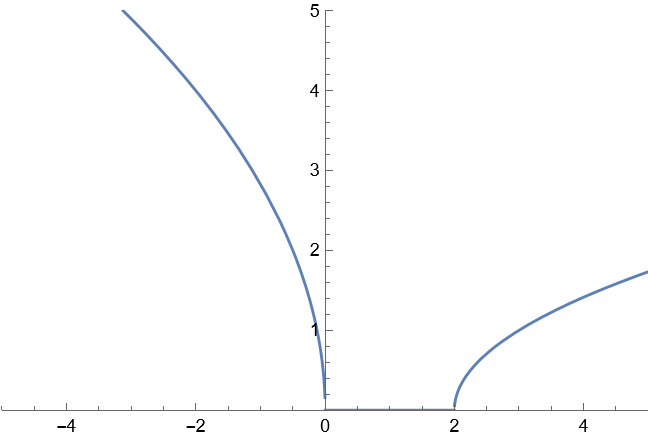
\includegraphics[width=\textwidth]{plot/dos-insulator.png}
        \subcaption{}
    \end{subfigure}
    \begin{subfigure}{0.45\textwidth}
        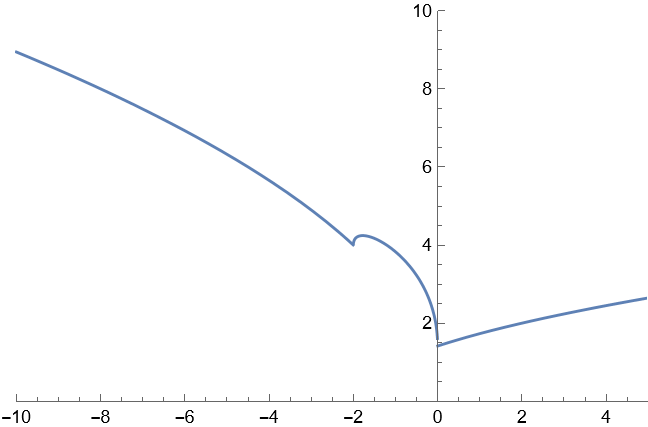
\includegraphics[width=\textwidth]{plot/dos-metal.png}
        \subcaption{}
    \end{subfigure}
    \caption{Density of state plots (a) Insulator (b) Metal}
    \label{fig:dos}
\end{figure}

When the conduction and valence bands are upward and downward dispersing parabolas 
centered around $\Gamma$,
the evolution of the DOS when we close the gap 
can be seen in \prettyref{fig:dos}.
In the insulating phase, 
there is a period where the DOS is exactly zero;
in the metal phase, 
there is a bump in the DOS curve 
corresponding to the overlap between the two bands.

In the insulating phase there is no conductivity,
because there is no active carrier:
the conduction band is completely empty;
the valence band contains no hole.
In the metallic phase we have 
\begin{equation}
    \sigma = \frac{n_{\text{e}} e^2 \tau_{\text{e}}}{m_{\text{e}}}
    + \frac{n_{\text{h}} e^2 \tau_{\text{h}}}{m_{\text{h}}}.
\end{equation}

\subsection{}

We consider a case in which phonons are ``frozen'' into a mean field, 
and the $\vb*{q}$ of that mean field is small compared 
wit the momenta of electrons.
We have
\begin{equation}
    X_i = \frac{1}{\sqrt{N}} \sum_q \ee^{\ii q a j} X_q , \quad 
    X_q = \sqrt{\frac{\hbar}{2 M \omega_q}} (b_q + b_{-q}^\dagger).
\end{equation}
Since $q$ involved here is small, 
in the system we have a lattice displacement field 
of a macroscopic wave length,
and the displacement field is almost constant in the eyes 
of electrons in a small region.
So if we use $X$ to refer to the displacement field in a small region, 
then we have 
\begin{equation}
    X = \frac{1}{\sqrt{N}} \sqrt{\frac{\hbar}{2 M \omega_0}} (b + b^*),
\end{equation}
where now $b$ is the (complex) mean field 
representing the phonon mean field.
Since $X$ is an intensive property,
it can be seen that $b \propto \sqrt{N}$.

The Hamiltonian is now 
(since the $U(1)$ symmetry is still kept, 
the chemical potential term has trivial behavior in diagonalization 
and can be left aside)
\begin{equation}
    \begin{aligned}
        H &= \sum_k \varepsilon^{\text{c}}_k c^\dagger_k c_k
        + \sum_k \varepsilon^{\text{v}}_k f^\dagger_k f_k 
        + \frac{g_0}{\sqrt{L}} \sum_k (b c^\dagger_k f_k + b^* f^\dagger_k c_k) \\
        &= \sum_k \pmqty{
            c^\dagger_k & f_k^\dagger
        } \pmqty{
            \varepsilon^{\text{c}}_k & \frac{g_0}{\sqrt{L}} b \\
            \frac{g_0}{\sqrt{L}} b^* & \varepsilon^{\text{v}}_k
        } \pmqty{
            c_k \\ f_k
        } .
    \end{aligned}
\end{equation}
Diagonalization of this Hamiltonian gives
\begin{equation}
    \varepsilon_k^{\text{c}', \text{v}'} = \frac{
        \varepsilon^{\text{c}}_k + \varepsilon^{\text{v}}_k 
        \pm \sqrt{
            (\varepsilon^{\text{c}}_k - \varepsilon^{\text{v}}_k)^2 
            + \frac{4 g_0^2}{L} \abs{b}^2
        }
    }{2}.
    \label{eq:diag-energy}
\end{equation}
It can be easily verified that 
the distance between the conduction band and the valence band is increased,
because when the square root in the expression is positive, 
it's larger than $\varepsilon^{\text{c}}_k - \varepsilon^{\text{v}}_k$.
Note that since $b \propto \sqrt{N} \propto \sqrt{L}$,
the above equation contains only intensive quantities 
and has no real $L$ dependence.

The ground state total energy is then 
\begin{equation}
    \begin{aligned}
        E' &= \sum_k \frac{
            \varepsilon^{\text{c}}_k + \varepsilon^{\text{v}}_k 
            - \sqrt{
                (\varepsilon^{\text{c}}_k - \varepsilon^{\text{v}}_k)^2 
                + \frac{4 g_0^2}{L} \abs{b}^2
            }
        }{2} + \hbar \omega_0 \abs{b}^2 \\
        &\approx \underbrace{\sum_k \varepsilon^{\text{v}}_k}_{E} 
        - \sum_k \frac{g_0^2}{(\varepsilon^{\text{c}} - \varepsilon^{\text{v}}_k) L} \abs{b}^2
        + \hbar \omega_0 \abs{b}^2.
    \end{aligned}
    \label{eq:ground-state-phonon}
\end{equation}
The second line only considers the $X^2$ term.
So whether creating a phonon coherent state in the ground state can save energy 
depends on the competition between 
the energy saving from dressing the electron 
with a phonon cloud 
and the energy cost to create some phonons.

The above results 
can also be found by many-body perturbation theory.
In the language of Feynman diagrams,
the irreducible self-energy diagram has exactly 
one $f^\dagger c$ vertex and one $c^\dagger f$ vertex, 
and we have 
\begin{equation}
    - \ii \Sigma_{k}^{\text{v}} (\omega)
    =\tikzset{every picture/.style={line width=0.75pt}} %set default line width to 0.75pt        
    \begin{tikzpicture}[x=0.75pt,y=0.75pt,yscale=-0.7,xscale=0.7, baseline=(XXXX.south) ]
    \path (0,100);\path (180.6666717529297,0);\draw    ($(current bounding box.center)+(0,0.3em)$) node [anchor=south] (XXXX) {};
    %Straight Lines [id:da48824437516573016] 
    \draw    (23.33,29.33) -- (68.83,29.33) ;
    \draw [shift={(49.88,29.33)}, rotate = 180] [fill={rgb, 255:red, 0; green, 0; blue, 0 }  ][line width=0.08]  [draw opacity=0] (8.93,-4.29) -- (0,0) -- (8.93,4.29) -- (5.93,0) -- cycle    ;
    %Straight Lines [id:da2397809827455355] 
    \draw    (68.83,29.33) -- (114.33,29.33) ;
    \draw [shift={(95.38,29.33)}, rotate = 180] [fill={rgb, 255:red, 0; green, 0; blue, 0 }  ][line width=0.08]  [draw opacity=0] (8.93,-4.29) -- (0,0) -- (8.93,4.29) -- (5.93,0) -- cycle    ;
    %Straight Lines [id:da5914746819325563] 
    \draw    (114.33,29.33) -- (159.83,29.33) ;
    \draw [shift={(140.88,29.33)}, rotate = 180] [fill={rgb, 255:red, 0; green, 0; blue, 0 }  ][line width=0.08]  [draw opacity=0] (8.93,-4.29) -- (0,0) -- (8.93,4.29) -- (5.93,0) -- cycle    ;
    %Straight Lines [id:da3532907307090305] 
    \draw  [dash pattern={on 0.84pt off 2.51pt}]  (68.83,29.33) -- (68.83,69.52) ;
    \draw [shift={(68.83,69.52)}, rotate = 135] [color={rgb, 255:red, 0; green, 0; blue, 0 }  ][line width=0.75]    (-5.59,0) -- (5.59,0)(0,5.59) -- (0,-5.59)   ;
    %Straight Lines [id:da06939704075217423] 
    \draw  [dash pattern={on 0.84pt off 2.51pt}]  (114.33,29.33) -- (114.33,69.52) ;
    \draw [shift={(114.33,69.52)}, rotate = 135] [color={rgb, 255:red, 0; green, 0; blue, 0 }  ][line width=0.75]    (-5.59,0) -- (5.59,0)(0,5.59) -- (0,-5.59)   ;
    % Text Node
    \draw (46.08,30.83) node [anchor=north] [inner sep=0.75pt]   [align=left] {$\displaystyle k$,v};
    % Text Node
    \draw (91.58,30.83) node [anchor=north] [inner sep=0.75pt]   [align=left] {$\displaystyle k$,c};
    % Text Node
    \draw (137.08,30.83) node [anchor=north] [inner sep=0.75pt]   [align=left] {$\displaystyle k$,v};
    \end{tikzpicture}
    = \frac{- \ii g_0 b}{\sqrt{L}} \cdot \frac{\ii}{\omega - \varepsilon^{\text{c}}_k + \mu}
    \cdot \frac{- \ii g_0 b^*}{\sqrt{L}},
\end{equation}
\begin{equation}
    \Sigma^{\text{v}}_k(\omega) = \frac{g_0^2}{L} \abs*{b}^2 \frac{1}{\omega - \varepsilon^{\text{c}}_k}.
\end{equation}
Note that this self-energy is \emph{exact}.
Now the dispersion relation is given by
\begin{equation}
    \omega - \varepsilon^{\text{v}}_k + \mu - \frac{g_0^2 \abs*{b}^2}{(\omega - \varepsilon^{\text{c}}_k + \mu) L} = 0.
\end{equation}
It's equivalent to \eqref{eq:diag-energy}.

\subsection{}

The first correction to the free energy 
caused by phonons 
is proportional to $b^2 \sim X^2$,
and it's sign depends on the competition 
between the two terms in \eqref{eq:ground-state-phonon}.
This term is to be merged with the $(T - T_{\text{c}}) X^2$ term.
So if \eqref{eq:ground-state-phonon} saves energy in the end,
$T_{\text{c}}$ is higher, 
and therefore electron-phonon coupling enhances the existing structural instability;
if the opposite case is true -- \eqref{eq:ground-state-phonon} is greater than 
the old band theory ground state $E$ -- 
then $T_{\text{c}}$ goes down and it's more difficult for the structural instability to happen.

\printbibliography

\end{document}